\section{Spatial filtering}
\label{app:spatial}

In the focal plane of a lens,
the intensity of the beam profile corresponds
to its Fourier transform.
To be more precise,
in the Fraunhofer approximation
(which is valid in the focal plane)
we find the intensity of each point on the focal plane
to be the amplitude of its respective
spacial Fourier component \cite{QE}.
We can use this fact
in order to manipulate the beam profile;
to spatially filter it.
This method is based on the fact that
Gaussians go into Gaussians under Fourier transform.

The core principle is simple:
We start with a (Gaussian) wave.
A first lens images this wave
onto the focal plane.
In this plane we place a mask.
This mask performs an operation
on the Fourier components present in the plane.
A second lens collimates the now modified beam back.

One useful mask geometry is a pinhole --
also known as low-pas filter.
Noise and other impurities on the beam profile,
picked up along the optical path,
is represented by higher Fourier components.
With a pinhole --
with appropriate aperture diameter --
we can cut off these higher components
and keep only the basic Gaussian in the middle.
Figure~\ref{img:spatialfiltering} by Edmund optics
illustrates this filtering.

\begin{figure}
\centering
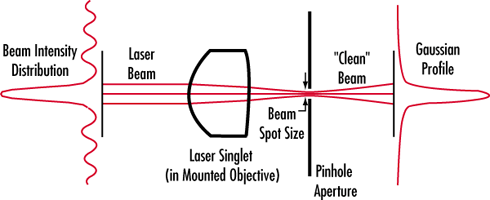
\includegraphics[width=12.5cm]{img/appendix/spatialfiltering.png}
\caption{Understanding Spatial Filters by Edmund optics \cite{Edmund}.}
\label{img:spatialfiltering}
\end{figure}

As already said,
the intensity in a point of the focal plane
is given by the amplitude
of its Fourier component $\nu_r$.
It is \cite{QE}
\begin{equation}
I = \left| \hat{g}(\nu_r) \right|^2,
\end{equation}
with $\hat{g}$ the Fourier transform
of a Gaussian beam
\begin{align}
g(r) &= \sqrt{I_0} \exp{\left(-\frac{r^2}{w_0^2}\right)}, \\
\hat{g}(\nu_r) &= \int r\d r\d \varphi g(r) \e^{i2\pi\nu_r r}\\
 &= \sqrt{I_0}\pi w_0^2 \exp{\left(-(\pi w_0 \nu_r)^2\right)}.
\end{align}
In the focal plane the Fourier component is given as
\begin{equation}
\nu_r = \frac{r}{\lambda f},
\end{equation}
with $\lambda$ the wavelength
and $f$ the focal length of the lens.
This results in an intensity distribution
\begin{equation}
I(r) = I_0(\pi w_0^2)^2 \exp{\left( -2(\frac{\pi w_0 r}{\lambda f})^2 \right)}.
\end{equation}
The fraction of power contained within diameter $D$ is hence \cite{Newport}
\begin{align}
\frac{P(r\leq \frac{D}{2})}{P_\mathrm{total}}
  &= \frac{2\pi}{P_\mathrm{total}} \int\limits_0^{D/2} I(r)r\d r \\
  &= 1- \exp{\left(-\frac{1}{2}(\frac{\pi w_0 D}{\lambda f})^2\right)}.
\label{eq:power}
\end{align}

A diameter of
\begin{equation}
D=\frac{f\lambda}{w_0}
\label{eq:diameter}
\end{equation}
permits $99.3\,\%$ of the total beam.
Newport \cite{Newport} recommends to use a pinhole
with this diameter.
Thorlabs on the other hand \cite{Thorlabs}
suggests to employ a pinhole
whose diameter is approximately $30\,\%$ larger.
The transmitted power in this case
would be $99.98\,\%$ of the total power.

By applying this method
to the output of a multi mode fiber,
we lose a considerable amount of this light;
the Gaussian part corresponds to TEM$_{0,0}$.
Starting with a Gaussian profile,
other methods can be used e.g.
to shape the beam into a super-Gaussian
\cite{Mansell2000},
in order to potentially
optimize the mode overlap.
